\chapter{Problematyka zagadnienia w świetle literatury}
\label{ch:problematyka}

\section{Charakterystyka choroby Parkinsona}
\label{sec:charakterystykaPD}
Choroba Parkinsona (PD) jest zwyrodnieniowym schorzeniem mózgu związanym z objawami motorycznymi (spowolnienie ruchowe,
drżenie, sztywność, zaburzenia chodu i równowagi) oraz szeroką gamą powikłań niemotorycznych (zaburzenia poznawcze,
zaburzenia psychiczne, zaburzenia snu oraz ból i inne zaburzenia sensoryczne).
Zaburzenia motoryczne, takie jak dyskinezy (ruchy mimowolne) i dystonie (bolesne mimowolne skurcze mięśni) przyczyniają
się do ograniczenia mowy, mobilności i ograniczeń w wielu dziedzinach życia.
Postęp tych objawów powoduje wysoki stopień niepełnosprawności i konieczność opieki.
U wielu osób z PD w trakcie trwania choroby rozwija się również demencja.

Ryzyko zachorowania na PD rośnie wraz z wiekiem, chociaż choroba może dotyczyć także młodszych osób.
Bardziej narażeni są mężczyźni niż kobiety.
Przyczyna PD nie jest znana, ale uważa się, że powstaje w wyniku złożonej interakcji pomiędzy czynnikami genetycznymi i
narażeniem na czynniki środowiskowe, takie jak pestycydy, rozpuszczalniki i zanieczyszczenia powietrza przez całe życie.

Według raportu Światowej Organizacji Zdrowia\cite{WHO} w skali globalnej niepełnosprawność i zgony z powodu PD
rosną szybciej niż w przypadku jakichkolwiek innych zaburzeń neurologicznych.
Częstość występowania PD podwoiła się w ciągu ostatnich 25 lat.
Globalne szacunki w 2019 roku wykazały ponad 8,5 miliona osób z PD.
Obecne szacunki sugerują, że w 2019 roku PD spowodowała 5,8 miliona lat życia z niepełnosprawnością, co
stanowi wzrost o 81\% od 2000 roku, i spowodowała 329 000 zgonów, co stanowi wzrost o ponad 100\% od 2000 roku.


[DODAĆ WYKRES]


W Polsce z chorobą Parkinsona zmaga się około 100 tys. pacjentów, z czego około 20\% jest już w stadium zaawansowanym
według informacji przekazywanych przez Fundację Chorób Mózgu.
Ponadto co roku w naszym kraju wykrywanych jest ok. 8 tys. nowych zachorowań.
Nowe zachorowania nadal skorelowane są z wiekiem, średnia wieku chorych wynosi 60 lat, niestety wzrasta odsetek chorych wśród osób młodych (nawet w wieku 20 lat).




\subsection{Etapy Choroby}
\label{subsec:etapypd}

Tu będę opierać się na tym\cite{Szurek_2018} i na tym\cite{Wieczorek_2013} i na tym\cite{Kuryłowicz_2019}

\subsection{Głos w chorobie Parkinsona}
\label{subsec:gospd}


\subsection{Problematyka choroby}
\label{subsec:problematykapd}


%---------------------------------------------------------------------------

\section{Przegląd dostępnych rozwiązań}
\label{sec:przeglad}

Diagnoza PD jest powszechnie oparta na obserwacjach lekarskich i ocenie objawów klinicznych, w tym charakterystyce różnorodnych objawów ruchowych.
Rosnąca liczba zachorowań i obniżenie wieku osób będących w grupie ryzyka, skutkuje wzrostem zainteresowania dotyczącym narzędzi, które ułatwiłyby
zarówno codzienne funkcjonowanie pacjentów jak i pracę lekarzy.
Tradycyjne metody diagnostyczne mogą być obarczone subiektywizmem ponieważ opierają się na ocenie ruchów, które są czasami subtelne dla
ludzkiego oka i dlatego trudne do sklasyfikowania, co może przyczynić się do błędnej diagnozy.
Ponadto wczesne objawy niemotoryczne PD mogą być łagodne oraz spowodowane wieloma innymi schorzeniami.
Dlatego też rozpoznanie tej choroby na wczesnym etapie stanowi wyzwanie.

Nie da się nie zauważyć, żę sztuczna inteligencja oraz nowoczesne technologie coraz częściej stają się integralną częścią systemu ochrony zdrowia.
Wspierają lekarzy podczas diagnozy oraz wyboru sposobu leczenia pacjenta,a także pozwalają na monitorowanie choroby.
Aby rozwiązać trudności i udoskonalić procedury diagnozowania oraz oceny PD, wdrożono metody uczenia maszynowego do klasyfikacji PD i osób zdrowych lub
pacjentów z podobnymi objawami klinicznymi (np. zaburzeniami ruchu lub innymi zespołami parkinsonowskimi).


W przeglądzie publikacji na temat wykorzystania uczenia maszynowego do diagnostyki PD do 2020 roku wyróżniono 209 artykułów\cite{ML_for_PD_review}.


\begin{figure}[htbp]
	\centering
	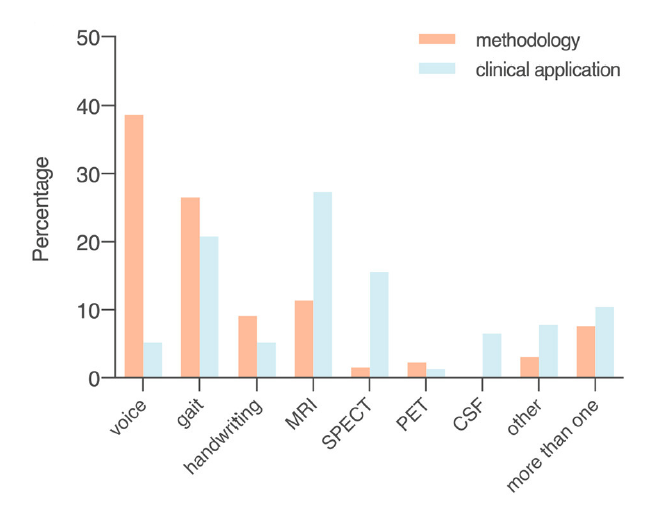
\includegraphics[width=0.5\textwidth]{./img/plot_PD_detection_methods}
	\caption{Wykres przedstawiający rozkład rodzaju danych na których bazowały systemy ML do diagnostyki PD\cite{ML_for_PD_review} (stan na dzień 14 luty 2020)}
    \label{fig:pd_detection_methods}
\end{figure}


\subsection{Rozwiązania teoretyczne}
\label{subsec:rozwiazania-teoretyczne}

\subsection{Aplikacje rzeczywiste}
\label{subsec:aplikacje}


\subsection{Niedopatrzenia dotychczasowych rozwiązań}
\label{subsec:wady_rozwiazan}

Ostatnie badania wykazały, że możemy wytrenować dokładne modele do wykrywania oznak PD z nagrań audio.
Jednakże, istnieją rozbieżności pomiędzy badaniami i mogą być spowodowane, częściowo, przez różnice w
wykorzystywanych korpusach lub metodologii.
Dlatego w  \cite{SustainedVowelsProblems} przeprowadzono analizę, wpływu niektórych czynników na wyniki klasyfikacji.
Głównym celem artykułu była ich identyfikacja oraz stworzenie zasad, które w przyszłosći pozwolą usystematyzować
stan wiedzy w tej dziedzinie.
W badaniach skupiono się na przedłużonych samogłoskach (ang. \emph{sustained vowels}), ponieważ jak wykazano wcześniej
[...].
Przeprowadzone eksperymenty wykazały, że nieuwzględnione zmienne w metodologii, projekcie eksperymentalnym i
przygotowaniu danych prowadzą do zbyt optymistycznych wyników w badaniach nad automatyczną detekcją PD.
Czynniki, które zidentyfikowano jako przyczyniające sią do zbyt optymistycznych wyników klasyfikacji
przedstawiono na Rys. \ref{fig:factors_PD_detection} oraz omówiono poniżej.


\begin{figure}[htbp]
	\centering
	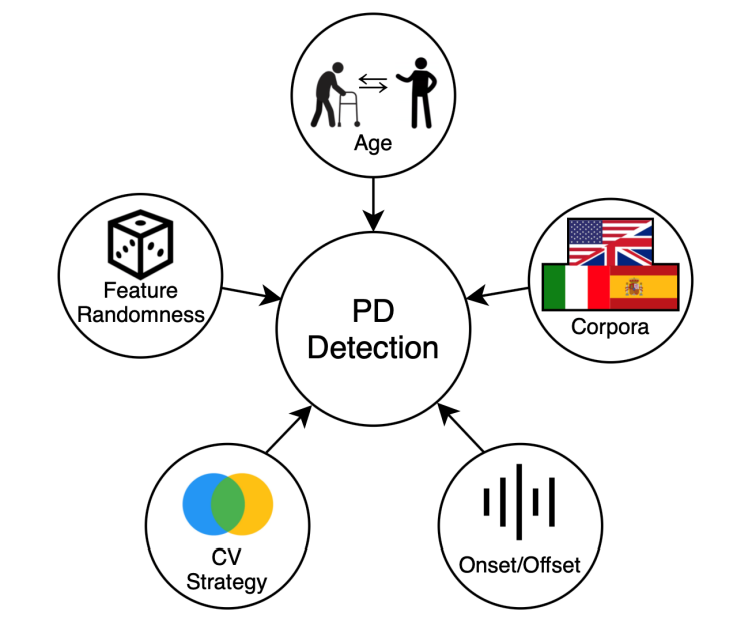
\includegraphics[width=0.4\textwidth]{./img/influence_of_factors_on_PD_detection}
	\caption{Czynniki wpływające na dokładność detekcji Parkinsona na podstawie głosu według analizy przeprowadzonej w \cite{SustainedVowelsProblems}}
    \label{fig:factors_PD_detection}
\end{figure}


\begin{enumerate}[label={\alph*)}]
	\item \textbf{Wpływ tożsamości mówcy}
	\item[] W przypadku, gdy w zbiorze danych znajduje się kilka nagrań od tego samego mówcy można postąpić na dwa sposoby.
Pierwszy z nich to podział według podmiotów (ang. \emph{subject-wise split}) polegający na tym, że nagrania od tej samej
osoby znajdują się albo w zbiorze treningowym albo testowym - nigdy w obu na raz.
W niektórych opracowań można spotkać też drugie podejście, czyli podział według rekordów (ang.\emph{record-wise split}), gdzie nagrania są losowo dzielone do zbiorów
lub intencjonalnie używa się nagrań od tej samej osoby zarówno w zbiorze testowym jak i treningowym.
Okazuje się, że podejście typu \emph{record-wise} prowadzi do wyższej dokładności niż \emph{subject-wise split}, jeśli pozostałe założenia pozostają identyczne.
Prawdopodobnie wynika to z faktu, że klasyfikator nastawia się na wykrywanie unikalnych informacji indywidualnych,
reprezentowanych przez współczynniki takie jak MFCC i PLP, a nie rzeczywiste biomarkery lub wzorce PD.
Dlatego też rekomendowana jest technika \emph{subject-wise split}, aby uniknąć zbyt optymistycznych wyników.

  	\item \textbf{Wpływ różnicy wieku między klasami}
	\item[] W literaturze można znaleźć prace wykorzystujące zbiory danych, w których  średni wiek mówców
w klasie osób chorych na PD różni się od średniego wieku w klasie osób zdrowych o ponad 5 lat.
Autorzy zapewniają o wysokiej skuteczności  swoich rozwiązań, jednak nie rozważają oni sytuacji, w której klasyfikator
uczy się wykrywać cechy powiązane z wiekiem, zamiast rzeczywistych wzorców PD.
Aby zbadać wpływ średniej różnicy wieku między dwiema klasami, w \cite{SustainedVowelsProblems} testowano różne przesunięcia rozkładu wieku.
Wraz ze wzrostem różnicy między średnim wiekiem uczestników z PD i HC, dokładność klasyfikacji konsekwentnie rosła (Rys. \ref{fig:acc_and_age_diff}).
Na tej podstawie można stwierdzić, że związany z wiekiem wpływ na głos mówców może zaburzać wyniki otrzymywane przez klasyfikator.
Dlatego też zaleca się zbilansowanie używanych zbiorów danych, tak aby średnia różnica wieku między dwoma klasami  była jak namniejsza.


\begin{figure}[htbp]
	\centering
	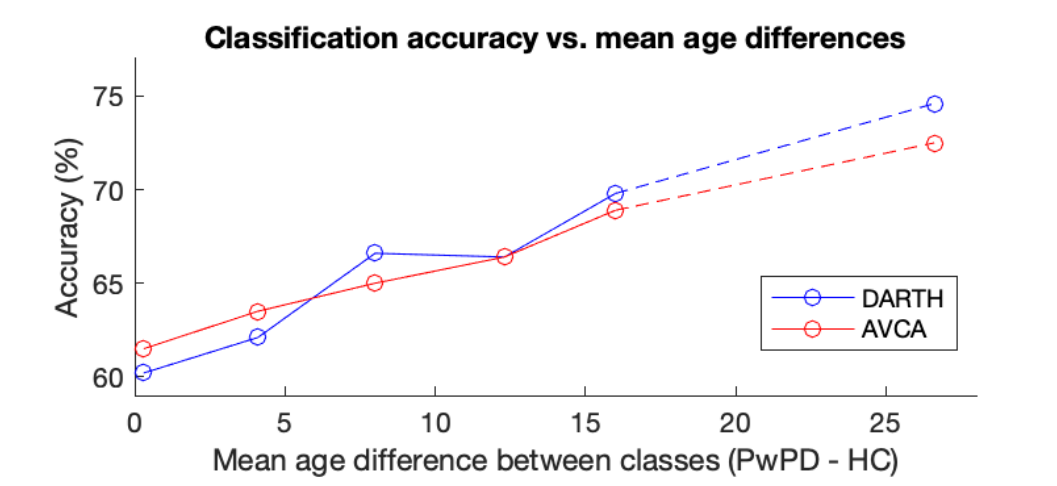
\includegraphics[width=0.7\textwidth]{./img/acc_and_age_difference}
	\caption{Wykres przedstawiający zależność różnicy wieku między klasami a dokładnością klasyfikacji \cite{SustainedVowelsProblems}}
    \label{fig:acc_and_age_diff}
\end{figure}

  	\item Wpływ losowości cech na dokładność klasyfikacji
	\item [] Im większa różnica między liczbą plików a wymiarem wektora cech, tym większe szanse na znalezienie cechy, która losowo koreluje z etykietami klas.
  	\item Łagodzenie losowego nadmiernego dopasowania przy użyciu danych programistycznych
	\item Wpływ rozpoczęcia i przesunięcia samogłosek na wyniki klasyfikacji
 	\item Eksperymenty międzykorporowe
	\item Analiza cech
\end{enumerate}



Nie są to jednak wszystkie czynniki, które zaburzają obiektywność wyników. Konieczna jest dyskusja na temat nowych
kompleksowych linii bazowych dla prowadzenia eksperymentów w automatycznym wykrywaniu PD na podstawie fonacji,
a także innych ogólnych zastosowań przetwarzania mowy.


\subsection{Wnioski}
\label{subsec:wnioski}

Prace nad automatyczną detekcją Parkinsona na podstawie głosu trwają już od dłuższego czasu.
Jednak wciąż brakuje systemu, który mógłby zostać uznany jako wystarczajaco niezawodne narzędzie diagnostyczne.
Wśród problemów, które ograniczają rzeczywiste wykorzystanie takich systemów wyróżnia się:

\begin{itemize}
\item pierwszy punkt
\item drugi punkt
\item trzeci punkt
\end{itemize}

%---------------------------------------------------------------------------
